\begin{frame}
 \frametitle{The \Qweak\ Experiment}
 \begin{block}{Event versus current mode}
  \begin{itemize}
   \item \alert{Event mode} (traditional)
    \begin{itemize}
     \item each electron individually registered
     \item event selection or rejection possible
    \end{itemize}
    \begin{center}
     \begin{tikzpicture}[scale=0.8]
      % Time axis and ticks
      \draw[->] (0,0) -- (6.5,0) node[below right]{time};
      \foreach \x/\xtext in {0/0,1/100\,ns,2/,3/,4/,5/,6/}{
       \draw (\x,0) -- (\x,-0.1) node[below] {$\xtext$};
      };
      % Current axis and ticks
      \draw[->] (0,0) -- (0,1.5) node[below left]{$\mu{}A$};
      % Photon pulse
      \foreach \x/\amp in {0.1/1.0,1.5/1.3,3.7/0.7,4.9/0.9}
       \draw[red,thick,shift={(\x,0)},yscale=\amp] plot[id=pulse,smooth,domain=0:1.5,samples=150]
        function {2.5*(x**(0.5))*((1+3*x/5)**(-10.0))};
     \end{tikzpicture}
    \end{center}
   \item \alert{Current or integrating mode}
    \begin{itemize}
     \item high event rates possible (event every nanosecond!)
     \item no suppression of background events possible
    \end{itemize}
    \begin{center}
     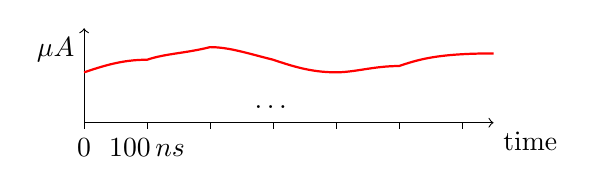
\begin{tikzpicture}[scale=0.8]
      % Time axis and ticks
      \draw[->] (0,0) -- (6.5,0) node[below right]{time};
      \foreach \x/\xtext in {0/0,1/100\,ns,2/,3/,4/,5/,6/}{
       \draw (\x,0) -- (\x,-0.1) node[below] {$\xtext$};
      };
      % Current axis and ticks
      \draw[->] (0,0) -- (0,1.5) node[below left]{$\mu{}A$};
      % Photon pulse
       \foreach \x/\amp in {0.1/1.1,0.25/1.2,0.31/0.9,0.43/1.0,0.51/1.1,0.57/1.1,0.73/1.0,0.79/1.1,0.92/1.1,1.1/1.1,1.25/1.2,1.31/0.9,1.43/1.0,1.51/1.1,1.57/1.1,1.73/1.0,1.79/1.1,1.92/1.1}
       \draw[thick,shift={(\x,0)},yscale=\amp] plot[id=pulse,smooth,domain=0:1.5,samples=150]
        function {2.5*(x**(0.5))*((1+3*x/5)**(-10.0))};
       \node at (3,0.25) {\ldots};
      % Average current
      \draw[red,thick]
       (0,0.8) .. controls (0.3,0.9) and (0.6,1.0) ..
       (1,1.0) .. controls (1.3,1.1) and (1.6,1.1) ..
       (2,1.2) .. controls (2.3,1.2) and (2.6,1.1) ..
       (3,1.0) .. controls (3.3,0.9) and (3.6,0.8) ..
       (4,0.8) .. controls (4.3,0.8) and (4.6,0.9) ..
       (5,0.9) .. controls (5.3,1.0) and (5.6,1.1) ..
       (6.5,1.1);
     \end{tikzpicture}
    \end{center}
  \end{itemize}
 \end{block}
\end{frame}
